%----------------------------------------------------------------------------------------
%	PACKAGES AND OTHER DOCUMENT CONFIGURATIONS
%----------------------------------------------------------------------------------------

\documentclass[11pt]{scrartcl} % Font size

%%%%%%%%%%%%%%%%%%%%%%%%%%%%%%%%%%%%%%%%%
% Wenneker Assignment
% Structure Specification File
% Version 2.0 (12/1/2019)
%
% This template originates from:
% http://www.LaTeXTemplates.com
%
% Authors:
% Vel (vel@LaTeXTemplates.com)
% Frits Wenneker
%
% License:
% CC BY-NC-SA 3.0 (http://creativecommons.org/licenses/by-nc-sa/3.0/)
% 
%%%%%%%%%%%%%%%%%%%%%%%%%%%%%%%%%%%%%%%%%

%----------------------------------------------------------------------------------------
%	PACKAGES AND OTHER DOCUMENT CONFIGURATIONS
%----------------------------------------------------------------------------------------

\usepackage{amsmath, amsfonts, amsthm} % Math packages

\usepackage{listings} % Code listings, with syntax highlighting

\usepackage[english]{babel} % English language hyphenation

\usepackage{graphicx} % Required for inserting images
\graphicspath{{Figures/}{./}} % Specifies where to look for included images (trailing slash required)

\usepackage{booktabs} % Required for better horizontal rules in tables

\usepackage{url}

\numberwithin{equation}{section} % Number equations within sections (i.e. 1.1, 1.2, 2.1, 2.2 instead of 1, 2, 3, 4)
\numberwithin{figure}{section} % Number figures within sections (i.e. 1.1, 1.2, 2.1, 2.2 instead of 1, 2, 3, 4)
\numberwithin{table}{section} % Number tables within sections (i.e. 1.1, 1.2, 2.1, 2.2 instead of 1, 2, 3, 4)

\setlength\parindent{0pt} % Removes all indentation from paragraphs

\usepackage{enumitem} % Required for list customisation
\setlist{noitemsep} % No spacing between list items

%----------------------------------------------------------------------------------------
%	DOCUMENT MARGINS
%----------------------------------------------------------------------------------------

\usepackage{geometry} % Required for adjusting page dimensions and margins

\geometry{
	paper=a4paper, % Paper size, change to letterpaper for US letter size
	top=2cm, % Top margin
	bottom=2cm, % Bottom margin
	left=2cm, % Left margin
	right=2cm, % Right margin
	headheight=0.75cm, % Header height
	footskip=1.5cm, % Space from the bottom margin to the baseline of the footer
	headsep=0.75cm, % Space from the top margin to the baseline of the header
	%showframe, % Uncomment to show how the type block is set on the page
}

%----------------------------------------------------------------------------------------
%	FONTS
%----------------------------------------------------------------------------------------

\usepackage[utf8]{inputenc} % Required for inputting international characters
\usepackage[T1]{fontenc} % Use 8-bit encoding

\usepackage{fourier} % Use the Adobe Utopia font for the document

%----------------------------------------------------------------------------------------
%	SECTION TITLES
%----------------------------------------------------------------------------------------

\usepackage{sectsty} % Allows customising section commands

\sectionfont{\vspace{6pt}\centering\normalfont\scshape} % \section{} styling
\subsectionfont{\normalfont\bfseries} % \subsection{} styling
\subsubsectionfont{\normalfont\itshape} % \subsubsection{} styling
\paragraphfont{\normalfont\scshape} % \paragraph{} styling

%----------------------------------------------------------------------------------------
%	HEADERS AND FOOTERS
%----------------------------------------------------------------------------------------

\usepackage{scrlayer-scrpage} % Required for customising headers and footers

\ohead*{} % Right header
\ihead*{} % Left header
\chead*{} % Centre header

\ofoot*{} % Right footer
\ifoot*{} % Left footer
\cfoot*{\pagemark} % Centre footer
 % Include the file specifying the document structure and custom commands

%----------------------------------------------------------------------------------------
%	TITLE SECTION
%----------------------------------------------------------------------------------------

\title{	
	\normalfont\normalsize
	\textsc{STAT 154: PROJECT 2}\\ % Your university, school and/or department name(s)
	\vspace{25pt} % Whitespace
	\rule{\linewidth}{0.5pt}\\ % Thin top horizontal rule
	\vspace{20pt} % Whitespace
	{\huge Daytime Arctic Cloud Identification Based on Multi-Angle Satellite Data\footnotemark[1]}\\ % The assignment title
	\vspace{12pt} % Whitespace
	\rule{\linewidth}{2pt}\\ % Thick bottom horizontal rule
	\vspace{12pt} % Whitespace
}

\author{Xiaoyang Wu (3034489979)  \\  Lanxin Zhang (3034487262)} % Your name


\date{\normalsize\today} % Today's date (\today) or a custom date

\begin{document}

\maketitle % Print the title
%------------------------------------------------

{\renewcommand{\thefootnote}{\*{*}}
\footnotetext[1]{\url{https://github.com/Gofinge/Daytime_Arctic_Cloud_Detection_Practice}}}

%----------------------------------------------------------------------------------------
%	Data Collection and Exploration
%----------------------------------------------------------------------------------------
\section{Data Collection and Exploration}
\subsection{Summary about the paper}

The paper \textit{Daytime Arctic Cloud Detection Based on Multi-Angle Satellite Data With Case Study} written by Shi et al. aims to provide a systematic method of accurate cloud detection in the Arctic which would do great favor to modulate the sensitivity of the Arctic and further, promotes the study on the dependence of surface air temperatures on increasing atmospheric carbon dioxide levels in the Arctic. The paper successfully identify three physically useful features--the linear correlation of radiation measurements from different MISR view directions (CORR), the standard deviation of MISR nadir red radiation measurements ($SD_An$) and a normalized difference angular index (NADI) and proposed two efficient operational Arctic cloud detection algorithms,\textbf{enhanced linear correlation algorithm (ELCA)} and \textbf{ELCM-QDA algorithm}, using \textbf{Multiangle Imaging SpectroRadiometer (MISR) images} provided by NASA, which yield satisfying outcome with high accuracy and coverage.\\

In achieving this, the vast amount of data provided by MISR is of vital importance. The MISR sensors comprise nine cameras viewing the Earth scene at nine distinct angles in four spectral bands and cover 233 paths extending across the daylight side of the Earth from the Arctic down to Antarcitica, collecting data from all paths on a repeat cycle of 16 days. The data used in the paper were collected form 10 MISR orbits of path 26, whose surface features are considerably rich, including the permanent sea ice, snow-covered and snow-free coastal mountains, permanent glacial snow and ice, and sea ice that melted during study period. These obits spans 144 days from April 28 to September 19 in 2002, which is exactly the daylight season in the Arctic. Among the 180 blocks in path 26, six data units 11-13, 14-16,17-19,20-22,23-25 and 26-28 are included, and 275-m red radiation measurement in the 26 measurements are chosen to investigate.\\

By comparing the performance of the two new algorithms to the expert labels, the researchers find out that the three physical features contain sufficient information to separate clouds from ice- and snow-covered surfaces and the algorithms are quite efficient.\\

The potential impact of this study is significant. First, the statistic methods used and the new algorithms proposed in this study provide inspiration for statisticians to think of appropriate and efficient methods in analyzing the abundant Earth science data that support weather and climate studies and also study fields beyond.  Second, in this study, statisticians are directly involved in data processing instead of joining after, which encourages statisticians to work directly together with other scientists and possible instrument team to achieve great success through close collaboration. Also, the result itself is of great influence, which provides strong statistic support to further study on dependences of surface air temperatures on increasing atmospheric carbon dioxide levels in the Arctic.

%------------------------------------------------

\subsection{Summary of data}
Combined three pictures together, the data in this project has \textbf{345556} observations and \textbf{11} features, including ten numerical variables and one class attribute variable. As for the class attribute variable \textbf{label}, we have 23.43\% observations labeled as \textbf{cloud}, 36.78\% observations as \textbf{not cloud}, and 39.79\% unlabeled. Also, in order to have a clear look at the distribution of different features, we draw histograms in figure 1.1, which shows that the five radiance angle all have negative skew. The relationship between the expert labels with the individual features will be discussed in the next subsection.\\

\begin{figure}
	\centering
	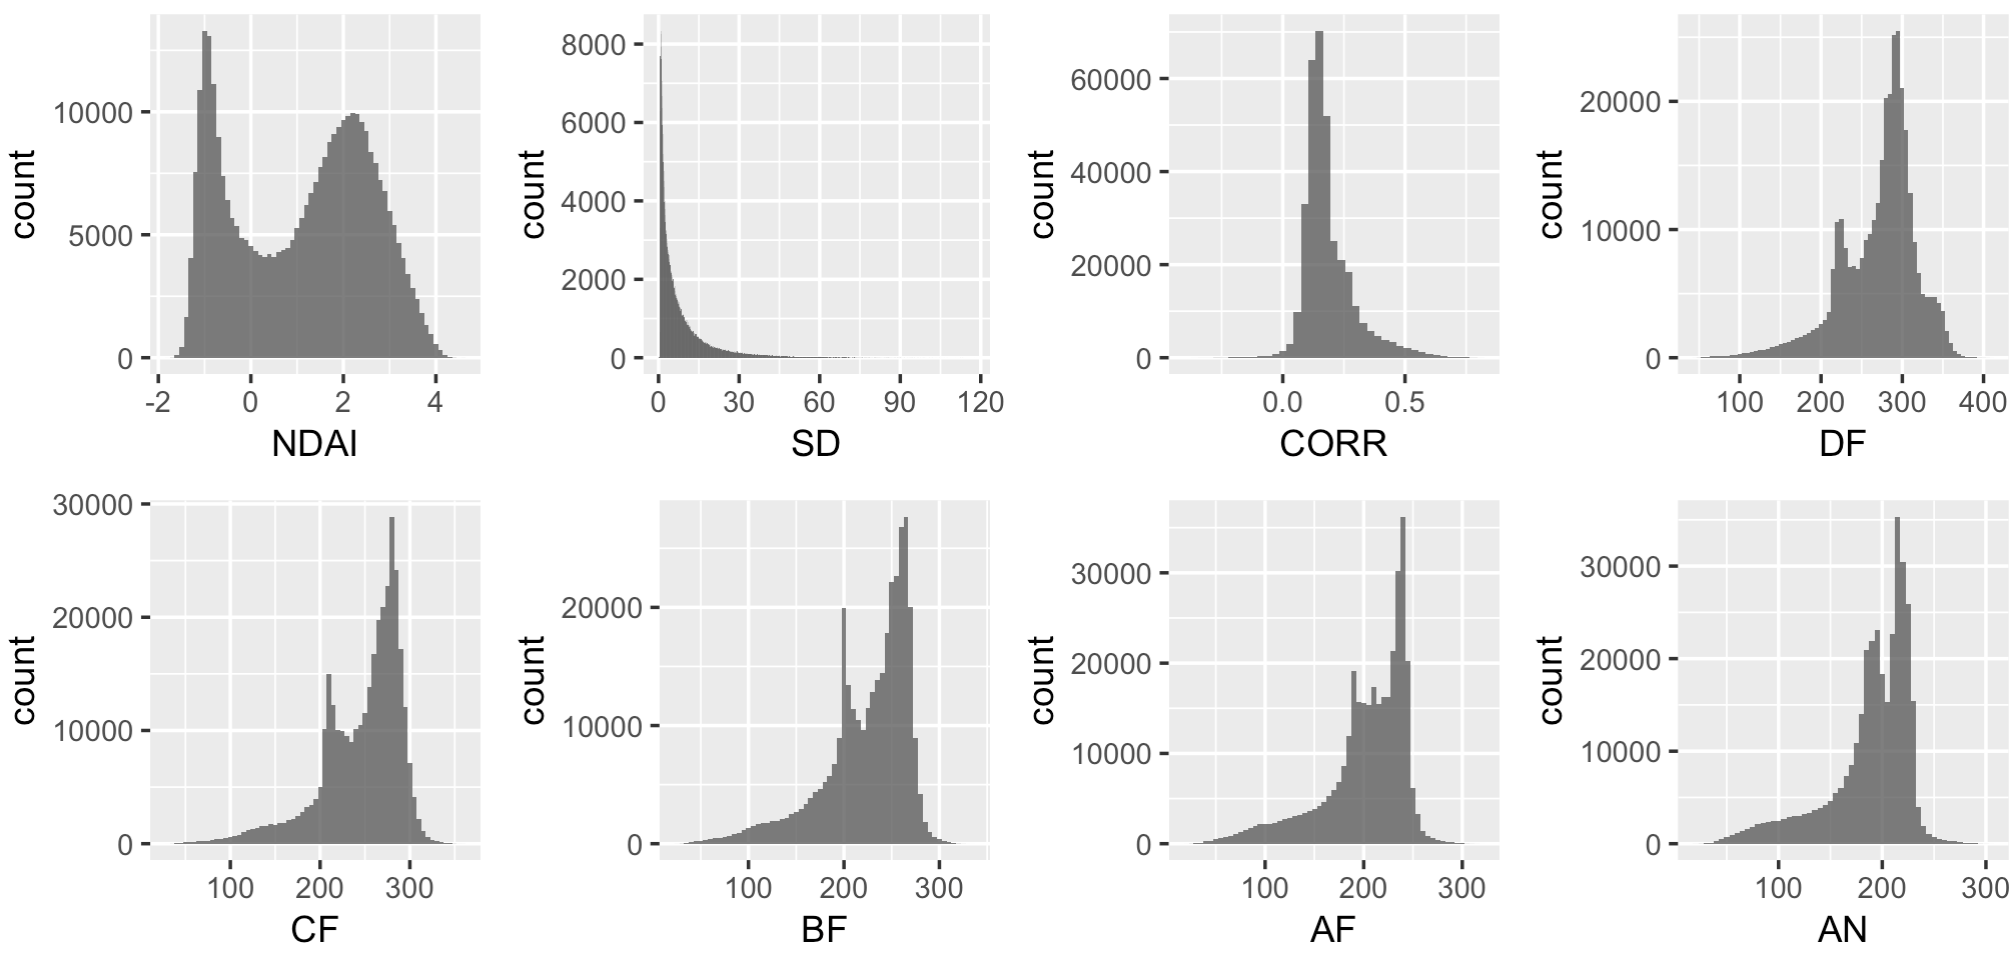
\includegraphics[width=0.6\columnwidth]{hist.png} % Example image
	\caption{Histograms of 8 features}
\end{figure}

\begin{figure}[htb]
	\centering
	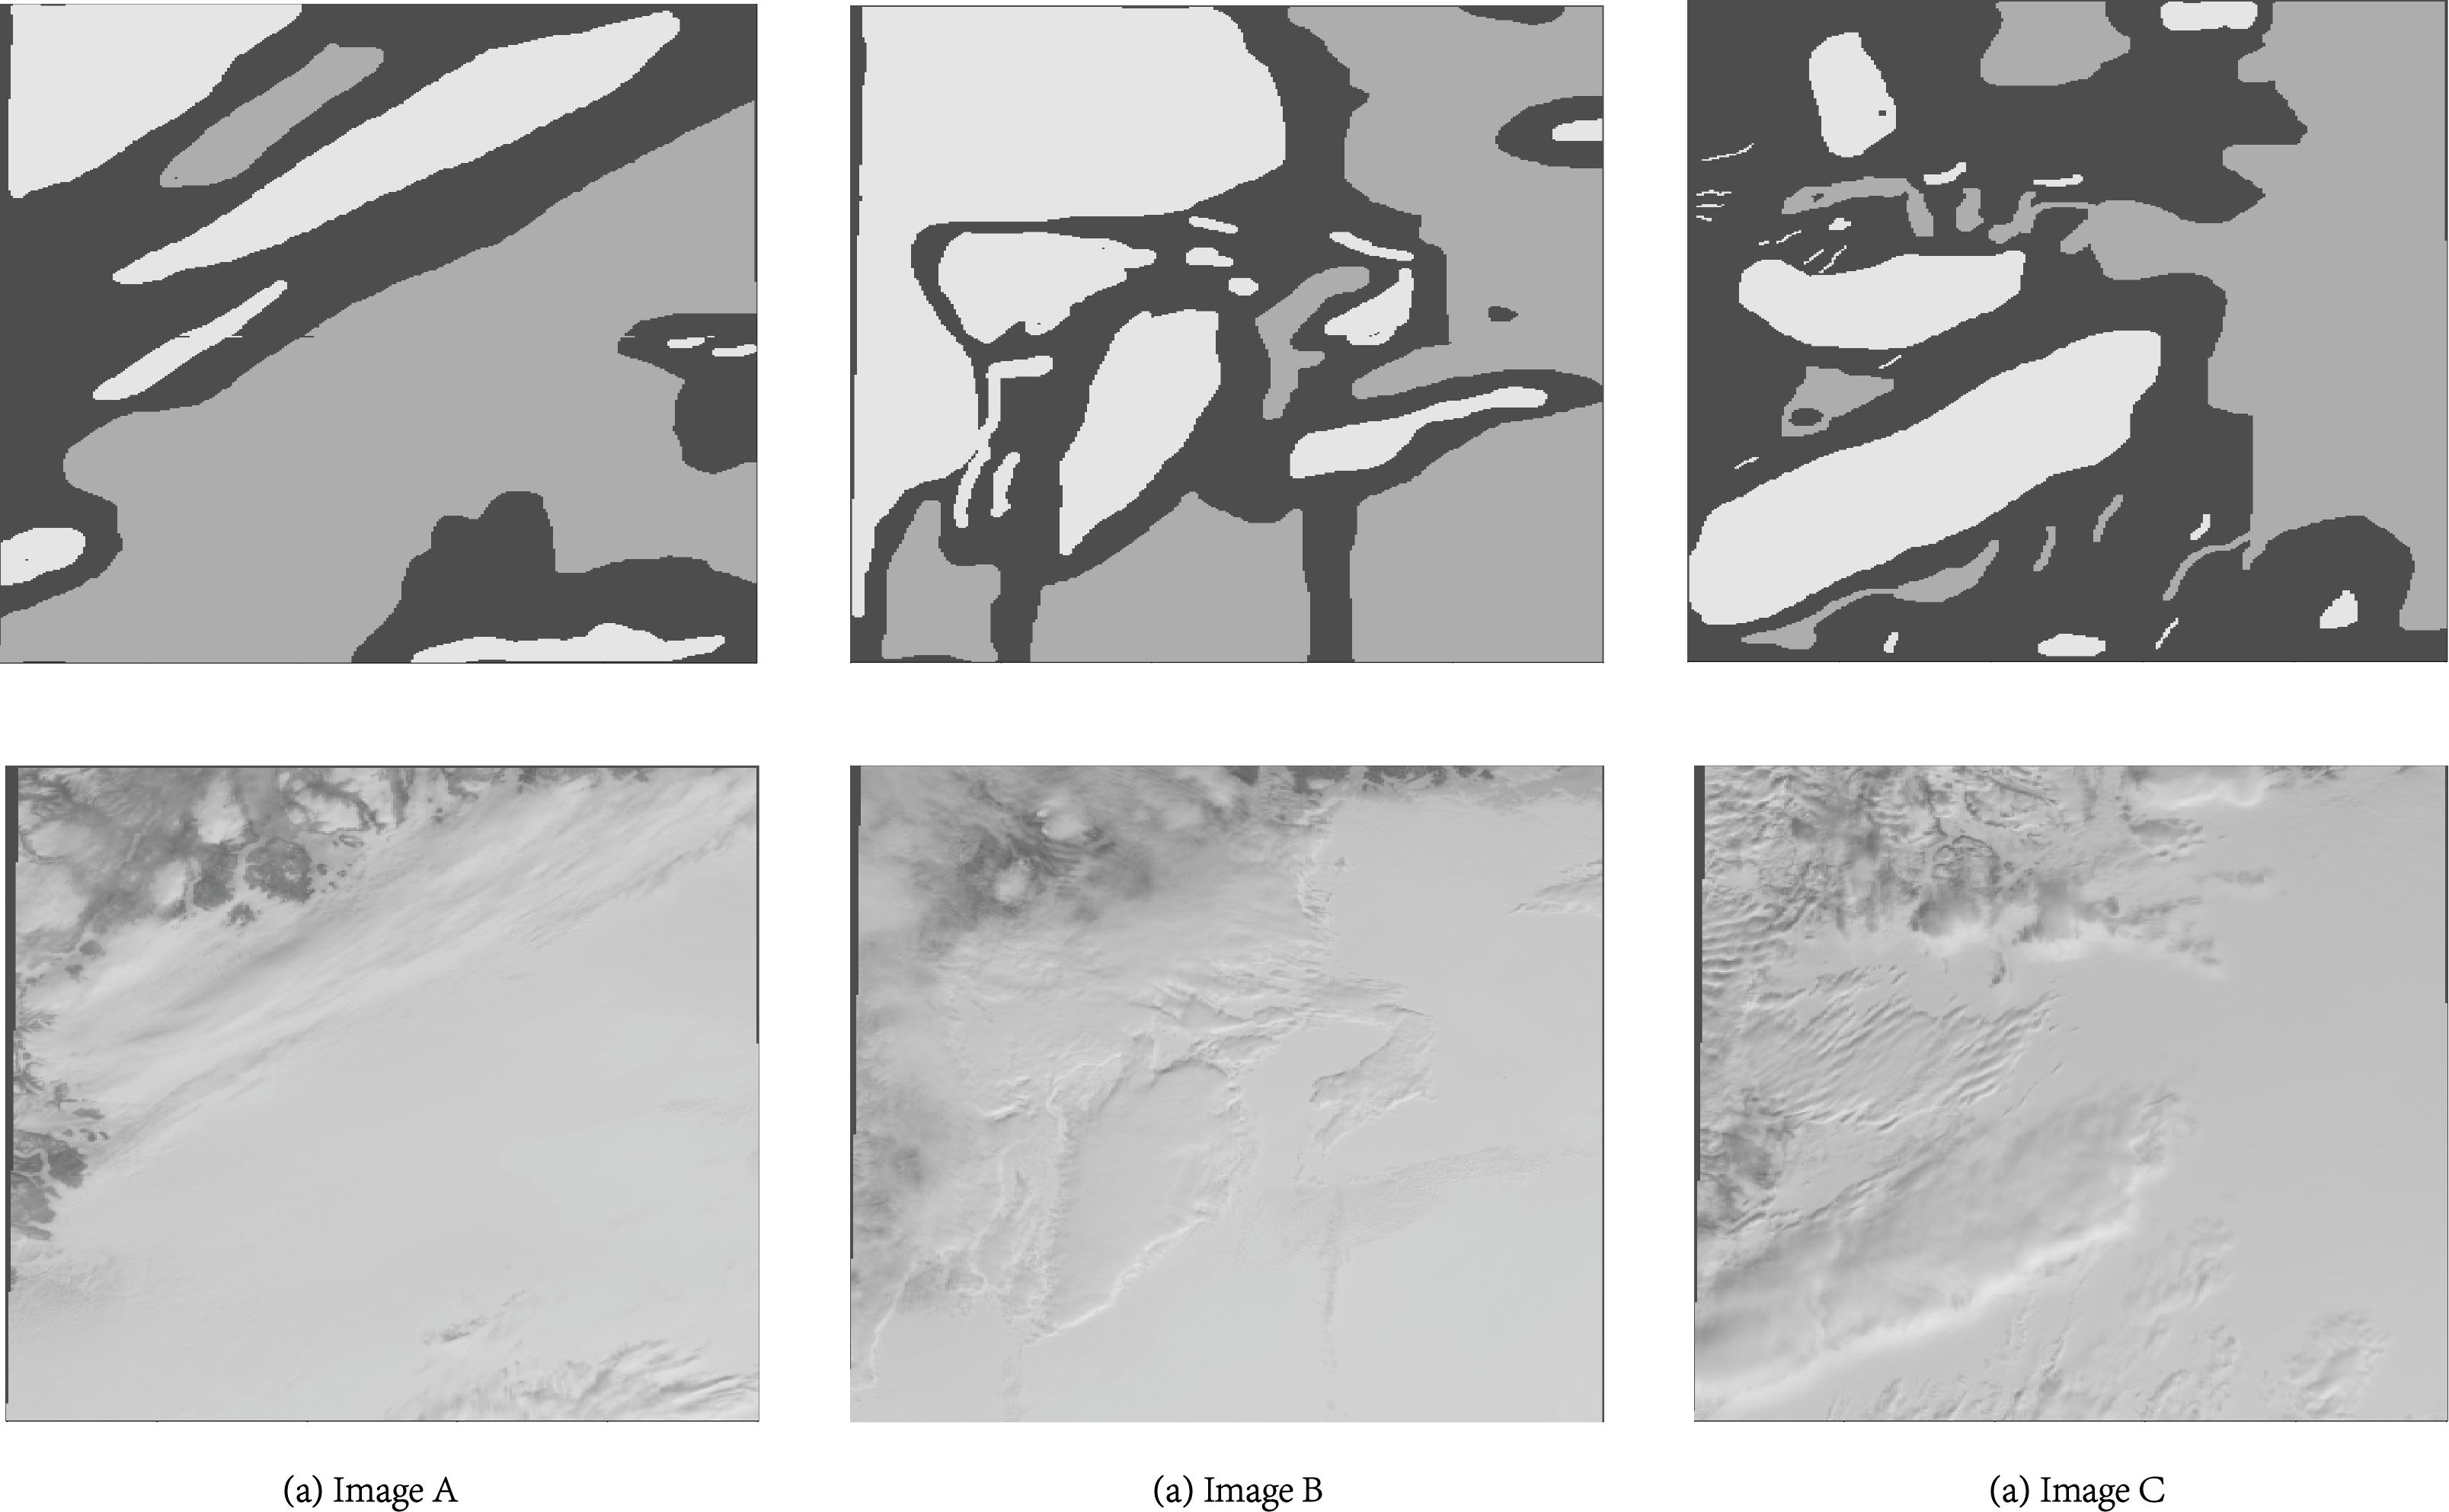
\includegraphics[width=0.6\columnwidth]{Image.png} % Example image
	\caption{Pixel images of data}
\end{figure}

In the labeled maps generating by x,y coordinates, as shown in Figure 1.2, we find out that pixels labeled as cloud and not cloud are well separated, and unlabeled pixels always occur between these two groups, which is natural since the pixels in boundary are always harder to classified. In this dataset, \textbf{the i.i.d assumption should not hold} since there seems to have strong correlation between neighbored pixels instead of existing independently.




%------------------------------------------------

\subsection{EDA of dataset}
In exploration of the dataset, we did some pairwise comparison between the features themselves by scatterplot and discussed the differences between two labeled classes in terms of the individual features by boxplots. Without loss of generality, we drawn 0.1\% of the total data randomly in order to better present the trends.\\

From figure 1.3 (boxplot), it is clear that there are some differences between two classes based on individual features. Namely, variables \textbf{y,x,DF,CF,BF,AF,AN} all yield higher values in pixels labeled as \textbf{not cloud} than those labeled as \textbf{cloud}, while variables \textbf{NDAI,SD,CORR} have lower values in \textbf{not cloud} group.

From figure 1.4 (pairwise), we can see that, ranking from strongest to weakest, y positively correlated with AF, AN, BF, CF, DF, negatively CORR; x positively correlated with AN,AF,BF,CF, negatively NDAI, CORR; NADI positively correlated with CORR, negatively AF,BF,AN; SD negatively correlated with AF,BF,AN,CF; CORR negatively correlated with AN,AF,BF; DF positively correlated with CF,BF,AF,AN. \\

Beside, we also have a rough look at the importance of these features by PCA. As showed in figure 1.5 (PCA), first three components contain almost 90\% of the variability of the data. We would discuss it in details in section 2.3.\\

\begin{figure}[htb]
	\centering
	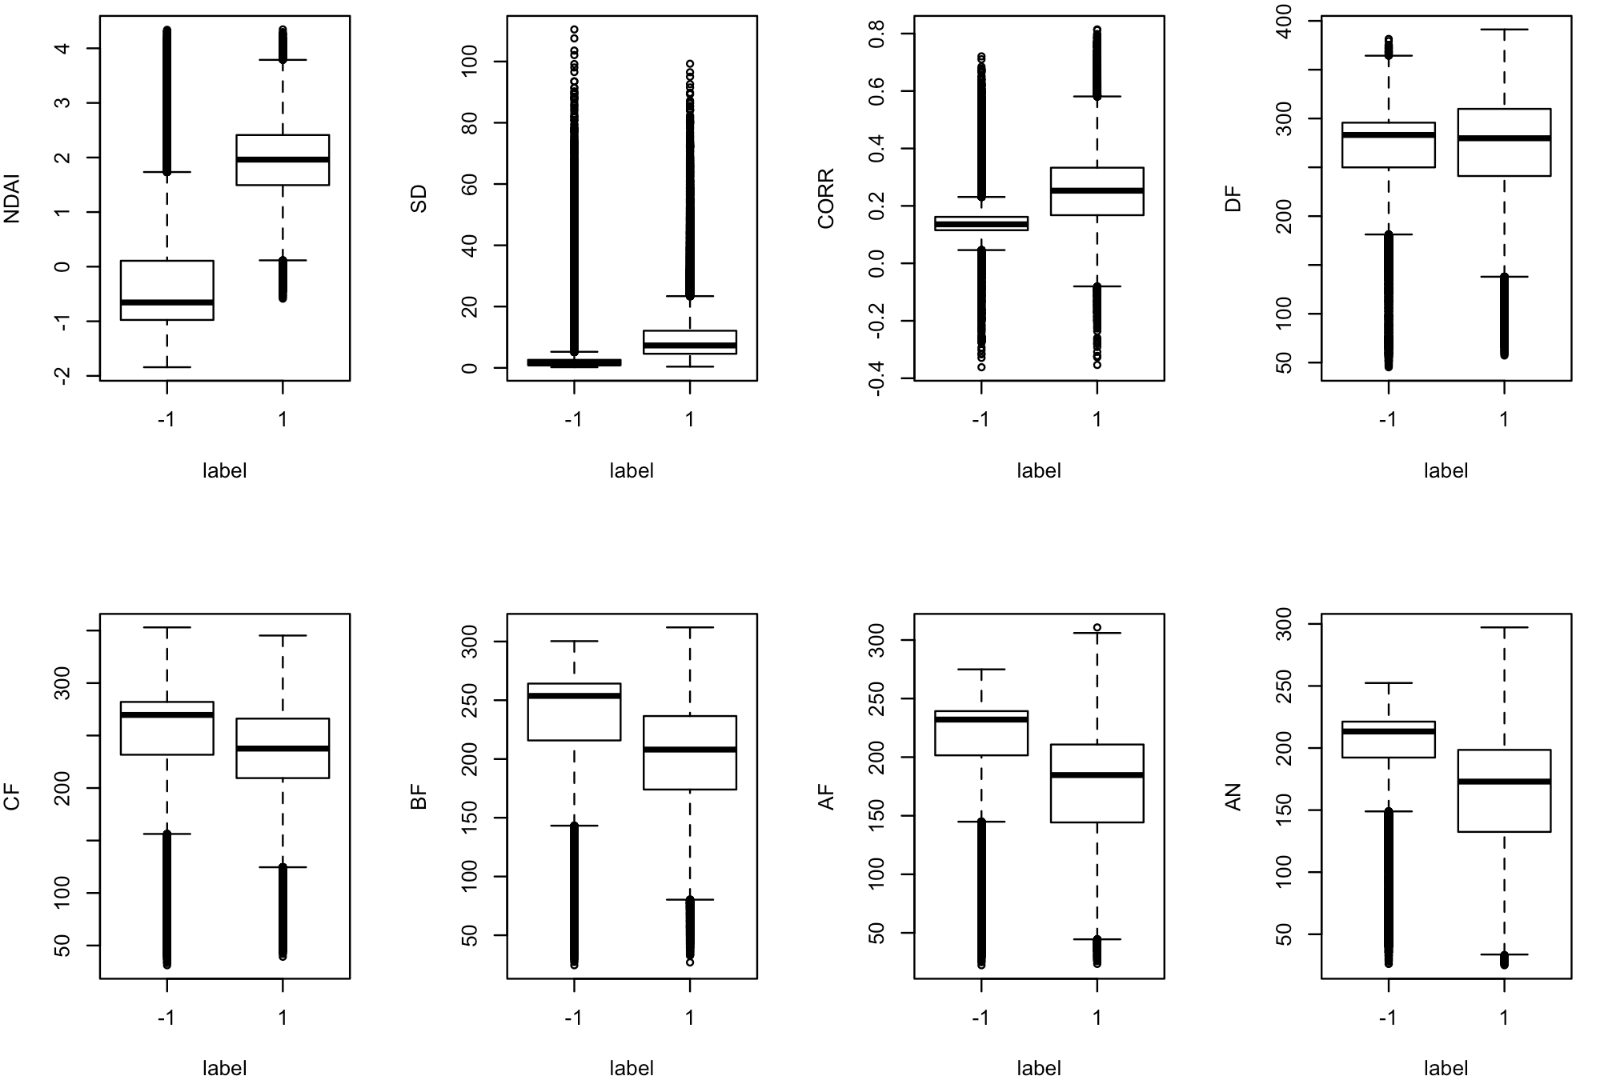
\includegraphics[width=0.6\columnwidth]{boxplot.png} % Example image
	\caption{Boxplot of features}
\end{figure}

\begin{figure}[htb]
	\centering
	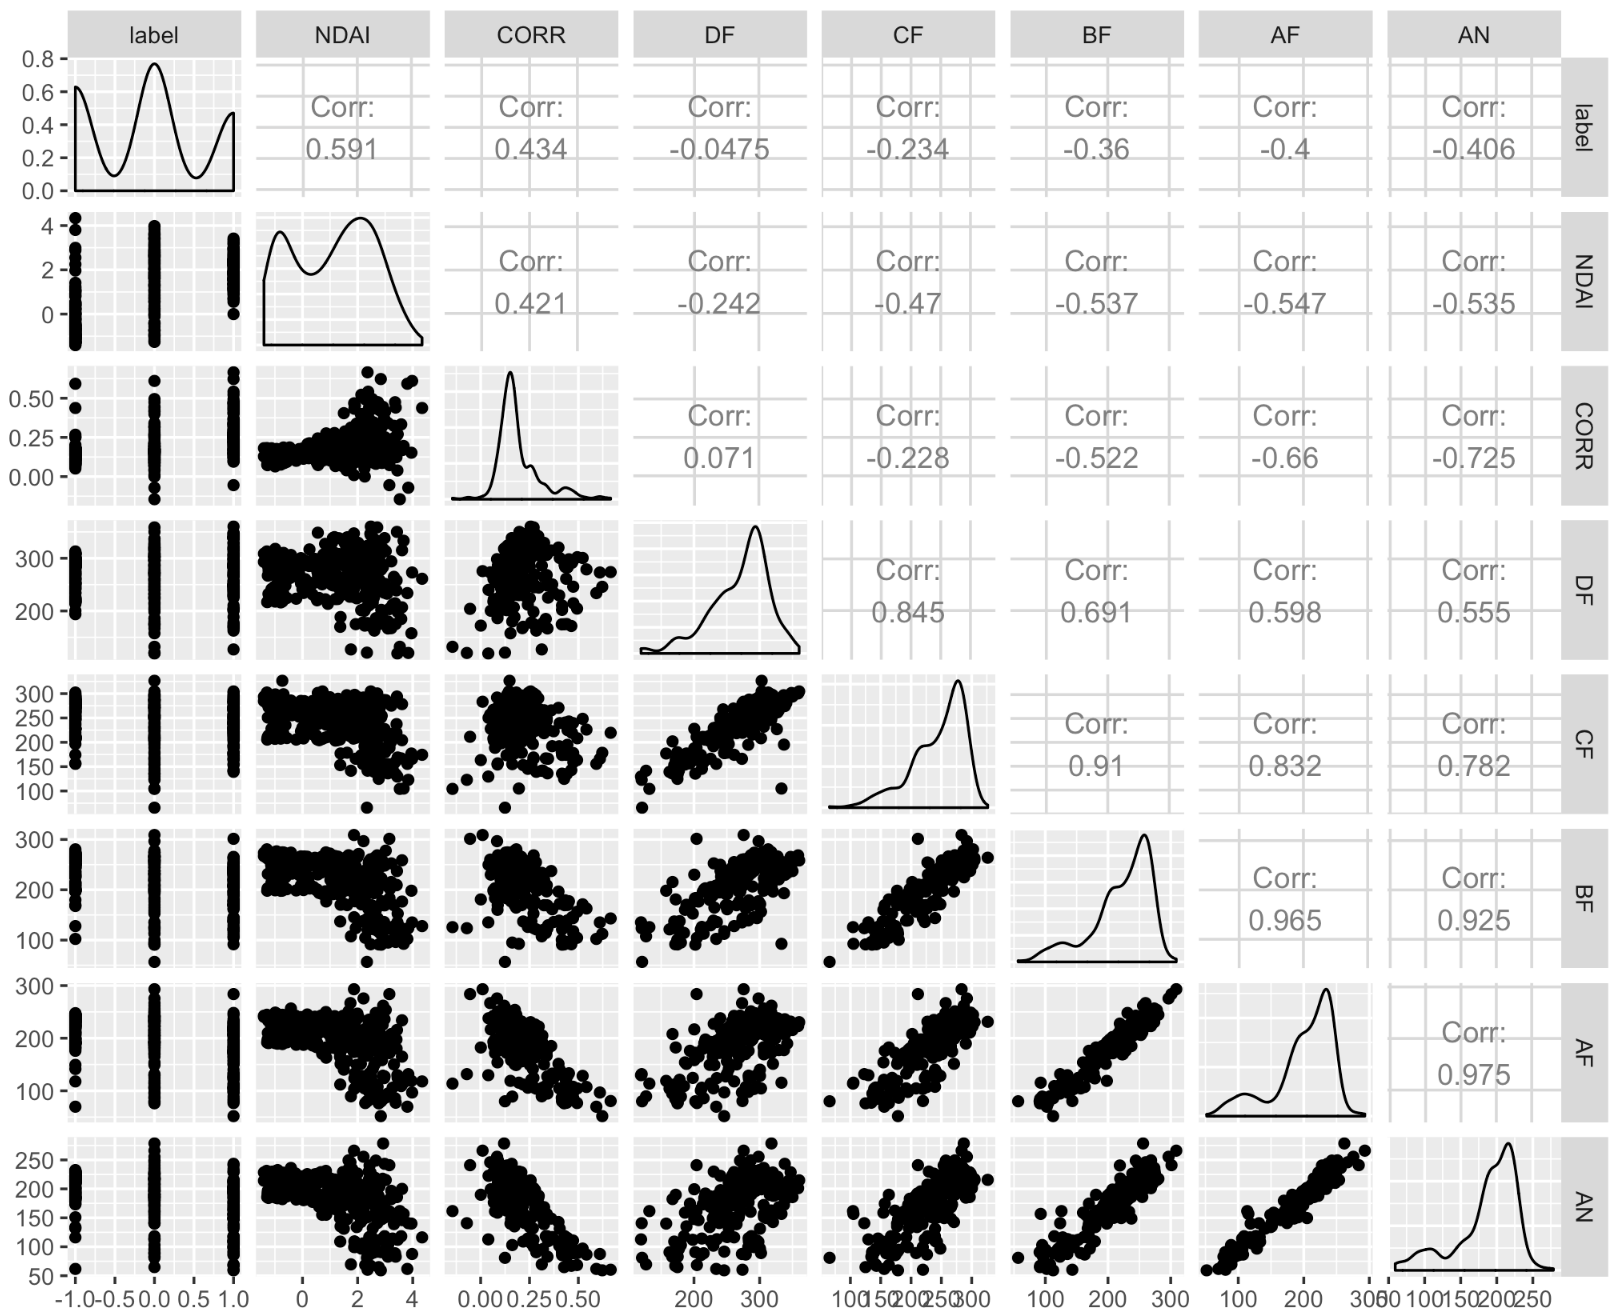
\includegraphics[width=0.6\columnwidth]{pair.png} % Example image
	\caption{Pair plot of data}
\end{figure}

\begin{figure}[h]
	\centering
	\includegraphics[width=0.6\columnwidth]{pca.png} % Example image
	\caption{PCA}
\end{figure}

%------------------------------------------------

%----------------------------------------------------------------------------------------
%	2. Preparation
%----------------------------------------------------------------------------------------

\section{Preparation}
\subsection{Splitting method}
Taking the invalid i.i.d assumption into consideration, we use two methods to split the data. The first method is \textbf{Average Grid Method(AGM)}. In this split,  we take $20\%$ of the total data as test set, $20\%$ as validation set and the rest as training set by picking pixels in every small grids which is divided by $x\cdot \sqrt{0.2} \times y\cdot \sqrt{0.2}$. \\

What's worth mentioning is that in order to make algorithm applied to all clouds picture instead of the specific three ones provided, we combine the data from the three pictures together instead of doing separately. With the same idea, we come up with the second split method, \textbf{Image Based Method (IBM)}, in which we take the second and third pictures as training set and then split first one to half-half randomly as test and validation set respectively. In this way, future data can be added by pictures in the training set and maintain their completeness.\\

As you can see, these two methods are of strong contradictory, since the former consider pixels individually and the latter consider pictures as a whole. We would discuss the performance of these two split methods in different classification ways and no surprisingly the former one yields higher accuracy. But in pragmatic situation, the latter one is more realistic, so we would take a further step to optimize the latter method in section 4. 

\subsection{Accuracy of trivial classifier}
The trivial classifier which sets all labels to -1 on the validation set and the test set yields an accuracy of \textbf{0.847} using QDA and accuracy of \textbf{0.864} using Logistic regression. The trivial classification seems unreasonable, but actually it would obtain relatively high average accuracy in some extreme scenario where the rate of pixels labeled as cloud is very small. 

\subsection{Best three Features}
In order to choose the "best" three features before modelling, we first apply PCA to the data. As showed in figure 1.5, the radiance angle features could classify the three groups clearly. But since the variance of five radiance angle features are much higher than CORR, NADI and SD, i.e $var[NDAI] = 2.02$ v.s. $var[AN] = 1627.80$. Thus the peripheral components ignored by PCA may also contain important information about the differences of data. Taking this into consideration, we turn to model based method to pick up features. As we can see from figure 2.1, the top three features in terms of importance yield by random forest, which perform best in classification in the next section are \textbf{NDAI,SD,CORR}.

\begin{figure}[htb]
	\centering
	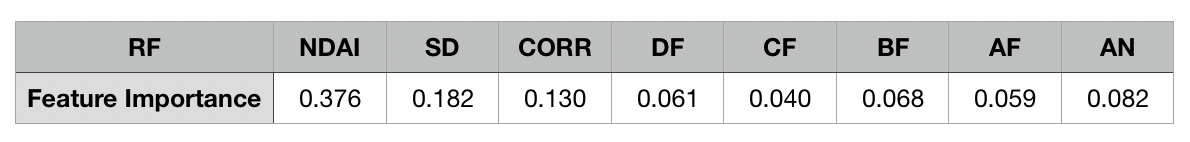
\includegraphics[width=0.6\columnwidth]{importance.png} % Example image
	\caption{Feature importance observed by Random Forest}
\end{figure}

\subsection{CVgeneric}
The generic cross validation function \textbf{CVgeneric} takes training features x, training labels y, number of folds k and loss function, which would return error rate, and default classifiers including QDA and Logistic regression as inputs, and K-fold CV loss on training set as well as the model as outputs.


%----------------------------------------------------------------------------------------
%	3. Modeling
%----------------------------------------------------------------------------------------

\section{Modeling}
In this section, we fit four different classification methods, including QDA, LDA, Logistic Regression (LR),and Random Forest into the data and assess their performance using cross-validation as well as ROC curves.\\

We have also tried KNN and SVM method but didn't fail to yield results efficiently due to the large computational cost while RF could be quickly performed in Python. The results show that random forest is ranked top both in accuracy and in ROC curves using the first splitting method and QDA obtain the highest accuracy using the second splitting method.\\

\subsection{Classification methods: assumption \& accuracy}
For different classification methods, we at first have a look at their assumptions: 

\begin{description}
\item [$\bullet$ LDA] assumes that the fitted data is Gaussian, and that each attribute has the same variance. 
\item [$\bullet$ QDA] assumes that the fitted data is Gaussian. 
\item [$\bullet$ Logistic regression] assumes

\begin{enumerate}
    \item The outcome is a binary or dichotomous variable.
    \item There is a linear relationship between the logit of the outcome and each predictor variables.
    \item There is no influential values (extreme values or outliers) in the continuous predictors.
    \item There is no high intercorrelations (i.e. multicollinearity) among the predictors.
\end{enumerate}

\item [$\bullet$ Random forest] assumes i.i.d
\end{description}

As we can see, all methods are based on the assumption of i.i.d. Since there do exist high correlations among predictors, as indicated in section 1, the fourth assumption of logistic regression is invalid. Also, since we can not guarantee the gaussian distribution of the data, the LDA and QDA would also have invalid assumption. \\

The accuracies across folds and the test accuracy for different methods using two splitting methods are shown in figure 3.1. It shows that  random forest is ranked top with accuracy 96.12\% and while the other three obtain similar accuracy using the first splitting method and in terms of the second split way, QDA obtain the highest accuracy of 88.28\% while Logistic regression yields the lowest 78.48\%.\\

\begin{figure}[htb]
	\centering
	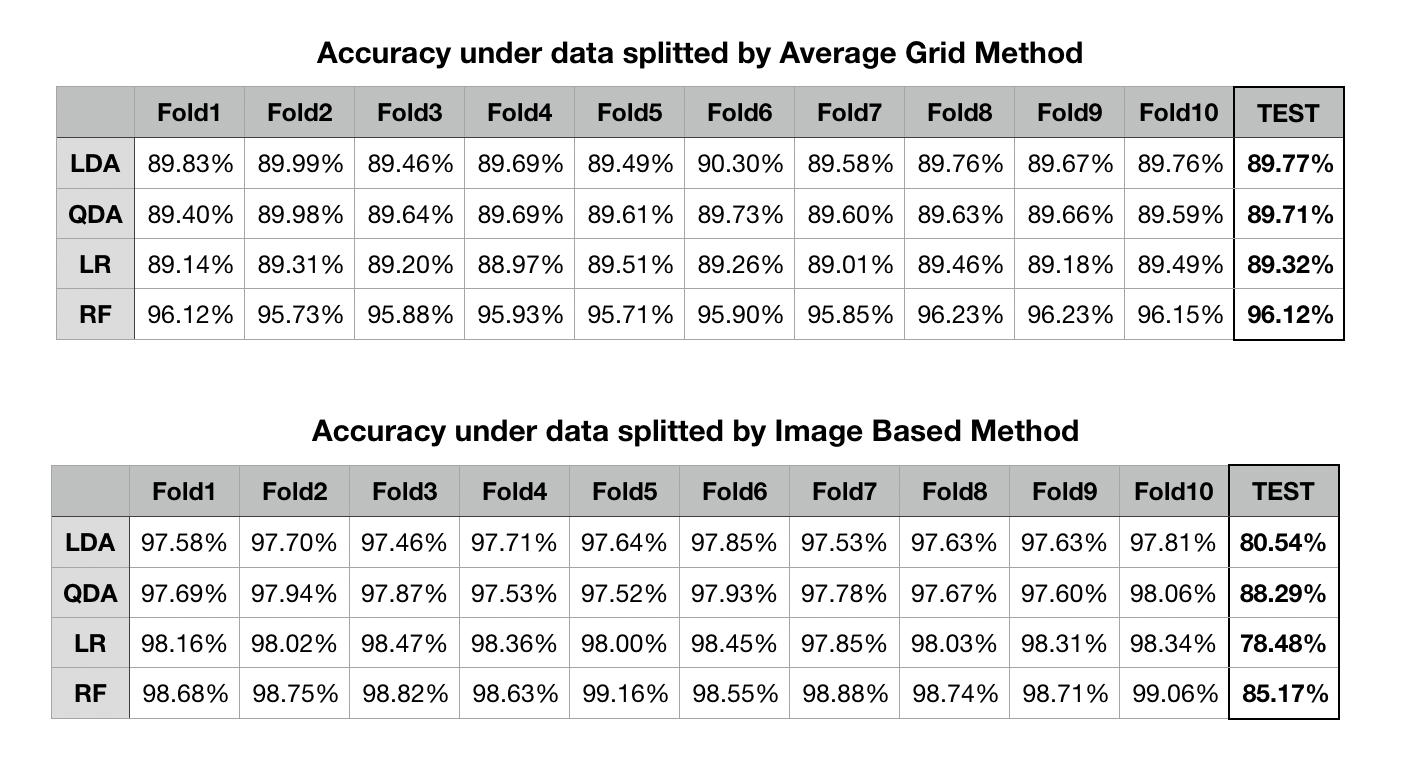
\includegraphics[width=0.8\columnwidth]{acc_table.png} % Example image
	\caption{Accuracy table of different classification under data splinted by two methods}
\end{figure}

\subsection{ROC curves}
In order to compare the performance of different classification methods directly, we use ROC curves in figure 3.2 to visualize the differences. Since the sensitivity (TPR) and miss rate (1 - FPR) should be weighed equally in this study, in order to balance the most top and most left, we perform the numeric differentiation on the values of each curve and choose the minimum of their absolute values after log transformation. In this way, we successfully identify the most left top ones in each curve, and it is clearly shown that the using both splitting way yield the same winner, random forest, whose curve is the nearest one to point (0,1), indicating that random forest perform best.\\

\begin{figure}[htb]
	\centering
	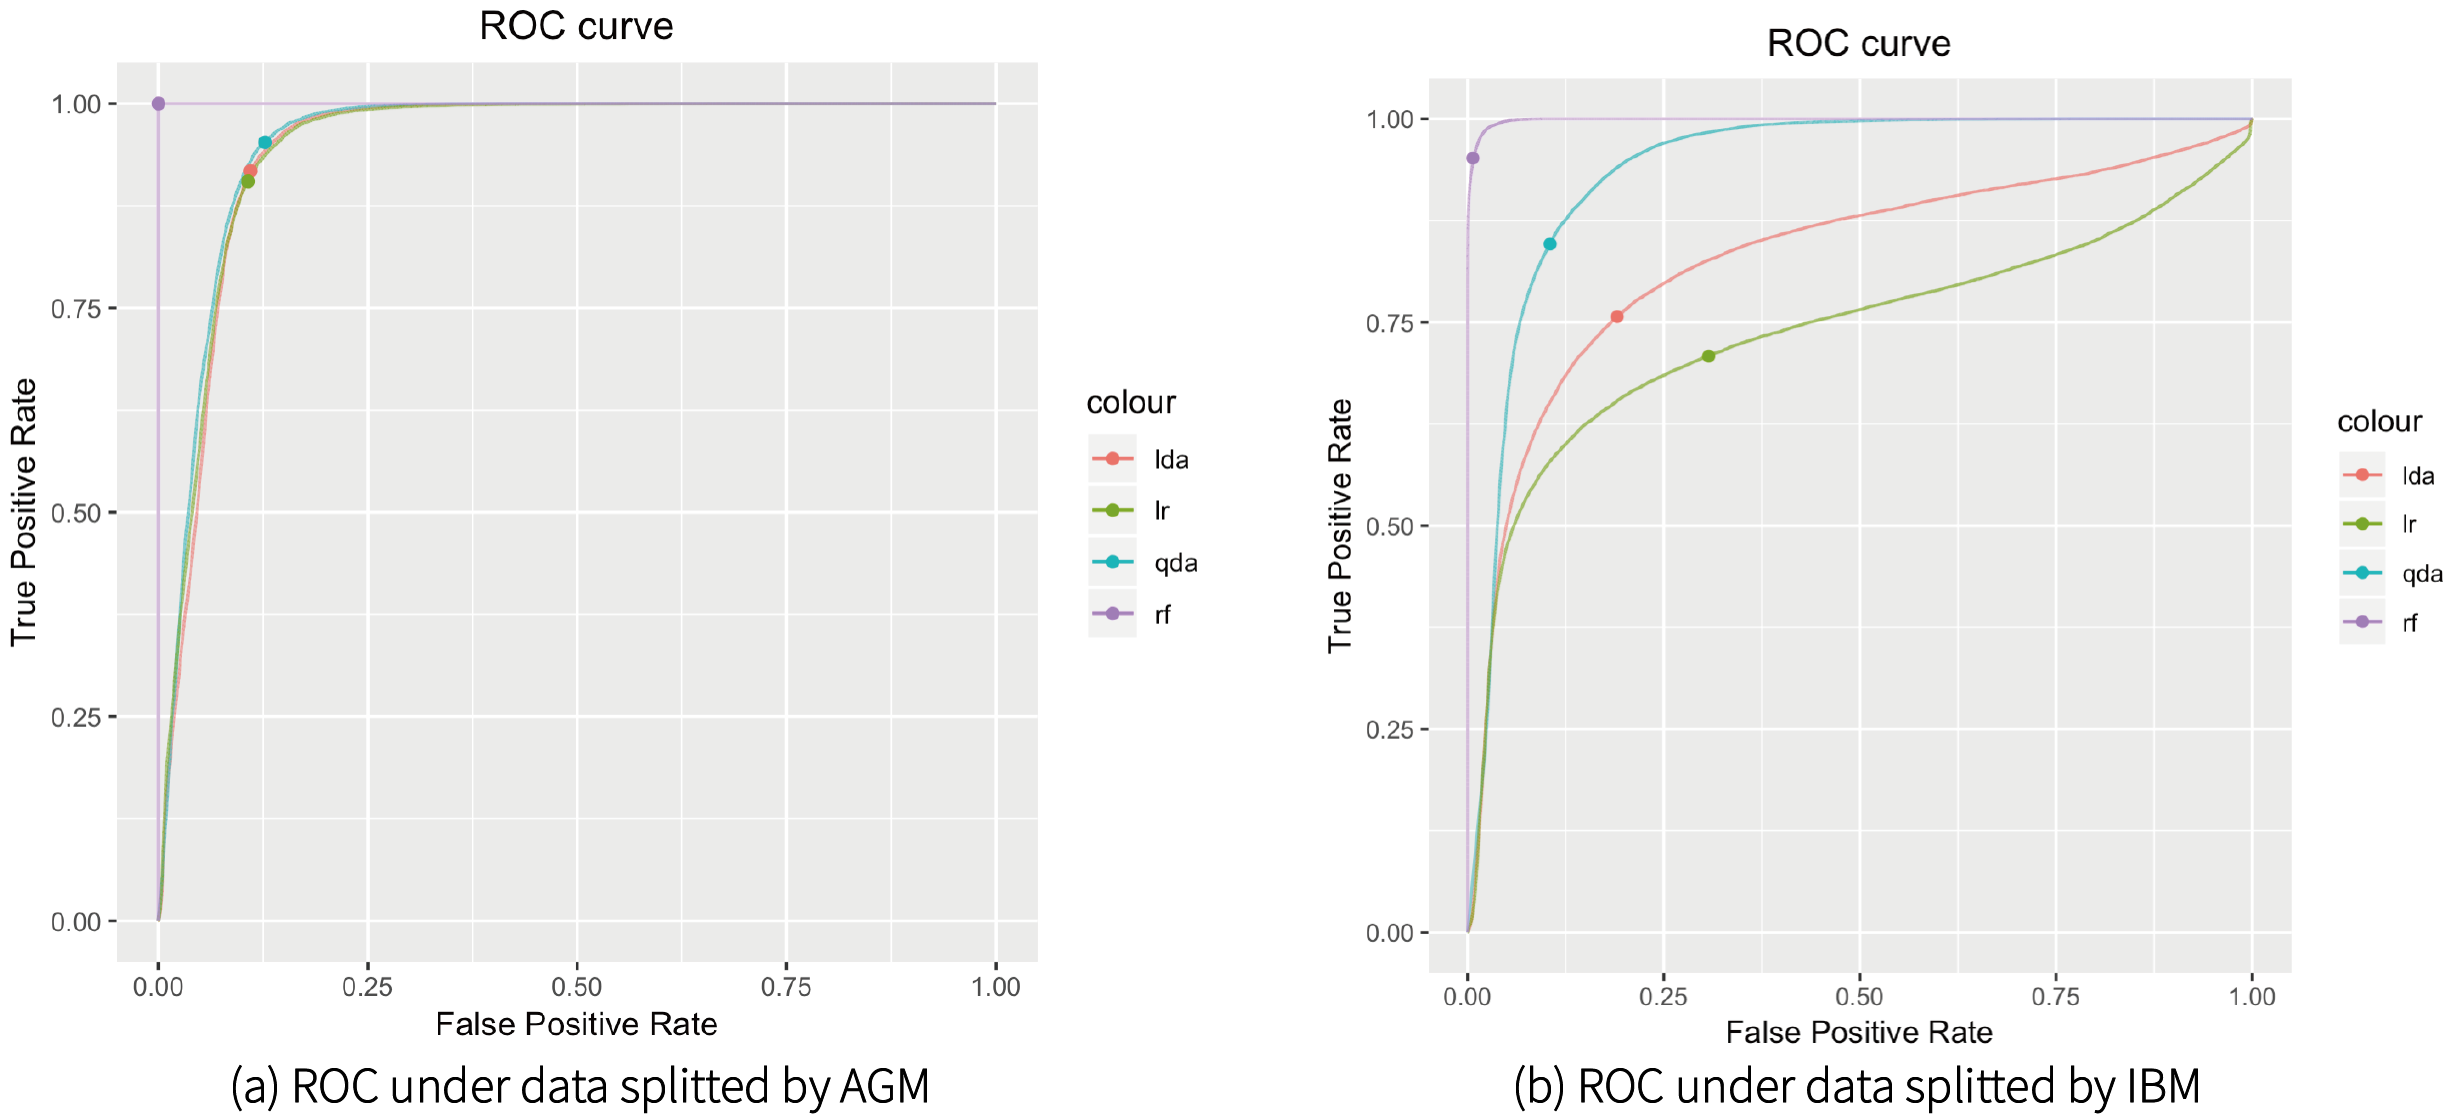
\includegraphics[width=0.8\columnwidth]{roc.png} % Example image
	\caption{ROC}
\end{figure}

\subsection{Another way to assess the fit}
Before discussing what kind of assessment should be claimed suitable to this problem, we design a figure to explain our consideration for the the assessment design.

As showed in figure 3.3, subfigure (c) is the label map for this designed case, (a) and (b) are two classification results with same error rate for this case. While the error rates for two classification are the same, the errors in result A occur randomly in all four regions and the errors in result B are all in the right bottom region, which corresponding to the two kinds of errors we would discuss in section 4.2. Since the second kind of errors are much harder to cope with and the first can be optimized by smoothing algorithm, we claim that result A is better than result B.

Keeping this in mind, we design a assessment of the fit to distinguish this two kind of errors even with same error rate, which first turn the classification results to matrix form via x-y axis and then use 2-norm values as criteria, the lower the value, the better the performance.

To put it mathematically, let $G(X)$ be the classification result matrix and $Y$ be the label map, the criteria value $S$ is obtained by:
$$S = \|G(X) - Y\|_2$$

As showed in Figure 4.3, we can see that by this new assessment criteria, random forest with errors randomly occuring are viewed better than QDA, whose errors mainly exis in a whole region, which verifies the effectiveness of our new assessment.

\begin{figure}[htb]
	\centering
	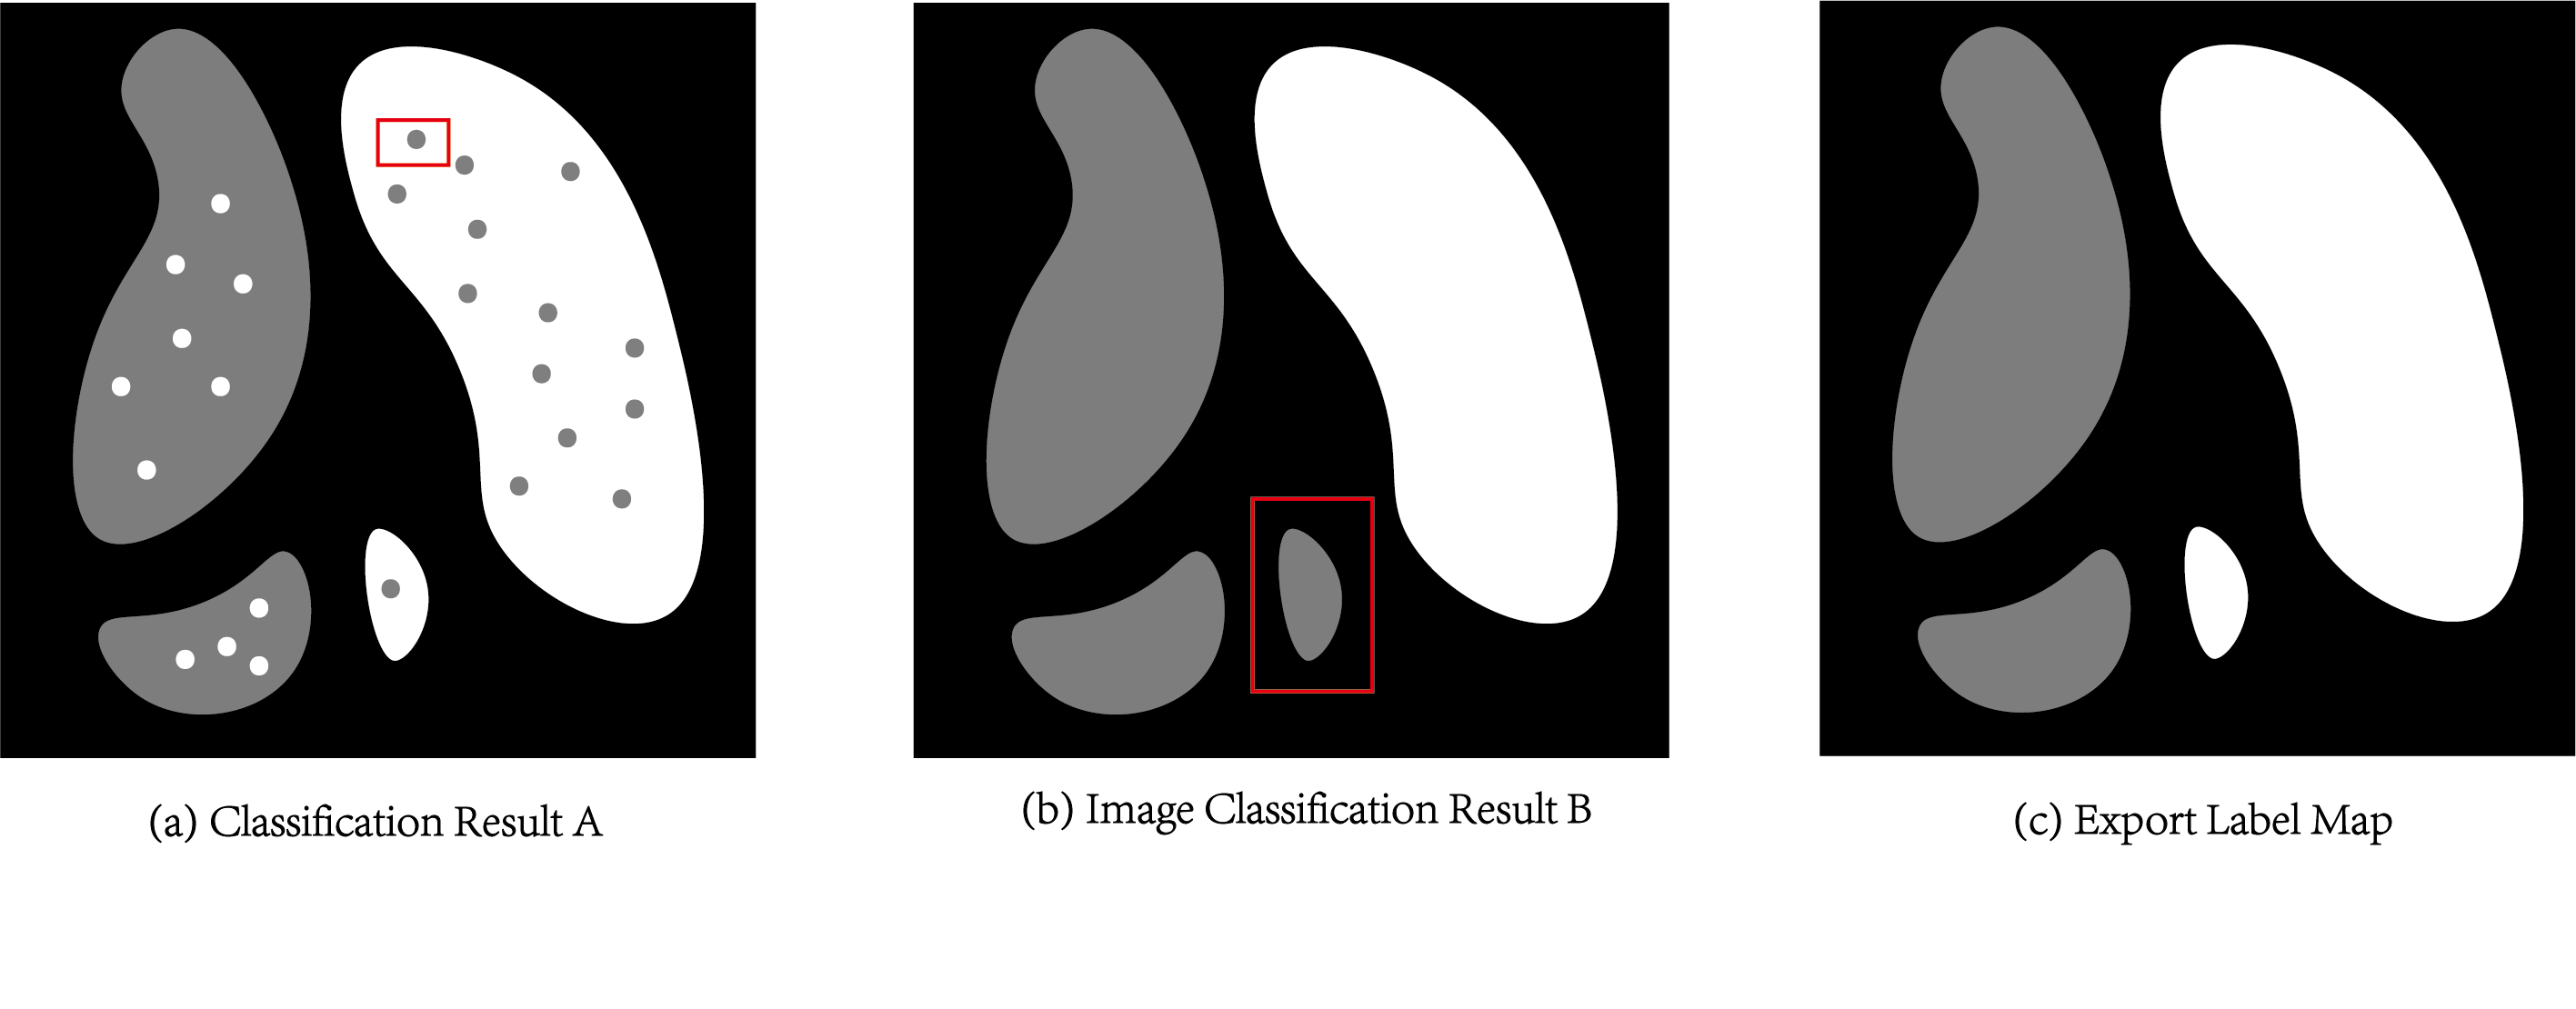
\includegraphics[width=0.8\columnwidth]{diagram.png} % Example image
	\caption{Example for two kinds of error}
\end{figure}

%----------------------------------------------------------------------------------------
%	4. Diagnostics
%----------------------------------------------------------------------------------------

\section{Diagnostics}
\subsection{In-depth analysis of a good classification model}
As we can see from sections above, random forest method perform extraordinarily in both accuracy (with test error as small as 0.03) and ROC curves compared with other classification method, which verify again the powerful strength that random forest have when applied to large dataset. In order to have a better understanding of its performance compared with the expert labels, we present the classification outcome in figure 4.1, where subfigure (a) shows the original expert labels, subfigure (b) shows classification performed by random forest without considering the unlabeled pixels, subfigure (d) predicts the unlabeled pixels as well and subfigure (c) is the real photo . As we can see clearly from figure 4.1, the classification results by random forest are almost the same as the expert labels. At the same time, the classification for unlabeled pixels are relatively reasonable to some extent compared with the real picture.

\begin{figure}[htb]
	\centering
	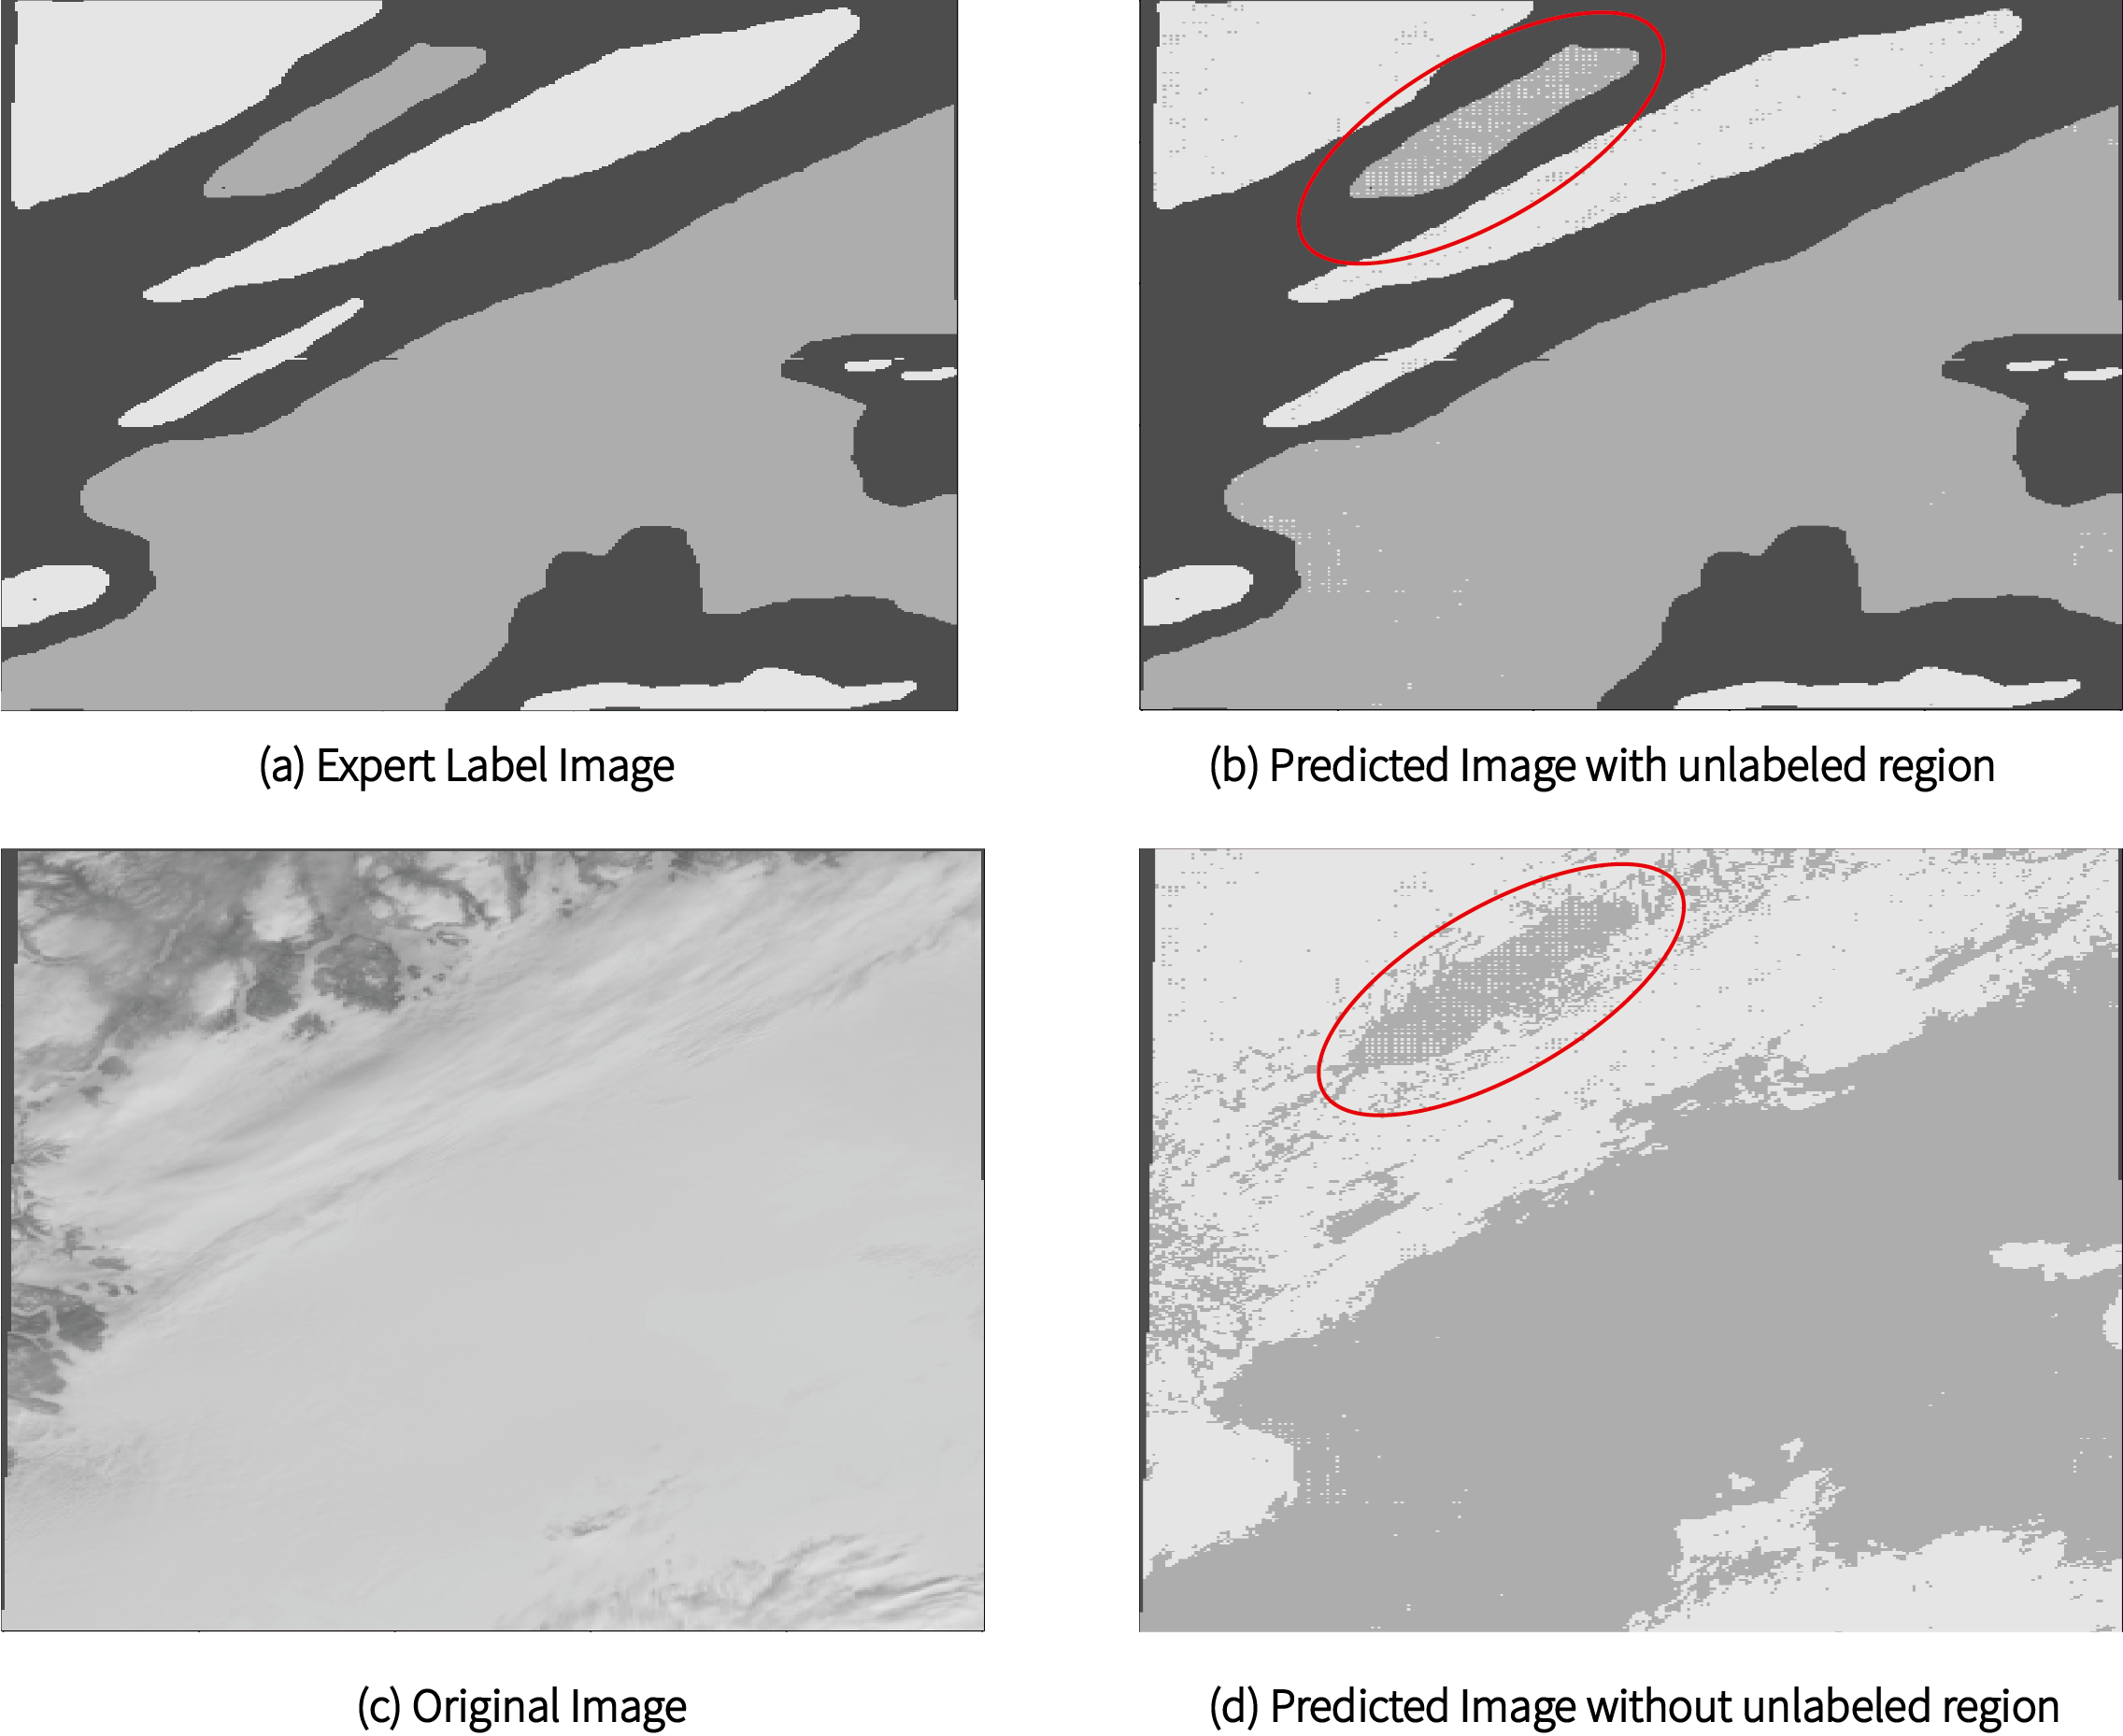
\includegraphics[width=0.6\columnwidth]{PoRF.png} % Example image
	\caption{Performance of Random Forest in data splitted by AGM}
\end{figure}




\subsection{Mis-classification errors}
Although the classification results using random forest algorithm are almost the same as the expert labels, there still exit two kinds of mis-classification errors. The first kind of errors occur mainly near the boundaries, which can be identified and revised by the optimized algorithm later in section 4.4, and the second kind of errors occur intensively in the a specific region, which is marked by red circle in Figure 4.1. In the region, the white small grids which should be gray in corresponding to the expert labels are exactly the pixels we picked as validation and test set according to our first splitting method —— average grid sample method. It would be more obvious in Figure 4.2 (a) using data splitted by IBM. What's worth mentioning is that, all the other classification fails in this region,which confirm our choice of random forest again, appearing white in the whole region which are labeled as gray by experts. The inconsistency between expert labels and classification results would be discussed later.

\subsection{Modify splitting way (answer of -d-)}
For a better reading experience, we move subsection (d) before (c) and discuss the splitting way first before analyzing the optimization of classifiers. \\

As we mentioned in section 2, the second splitting way -- Image Based Method -- should be a better choice considering the future application on more pictures and the non-i.i.d situation. The initial results of it, however, it's far from satisfactory, yielding accuracy of only 54.7\%. To investigate the reasons of the poor performance, we plot the histograms of features in three pictures provided and find there exist some linear deviation among pictures, which may be resulted by the difference of light intensification or other factors. Thus we normalized the features in three pictures and then obtain accuracy 85.2\%, still poorer than the first splitting method but closer to real life. \\

In this way, the comparison between this two splitting methods is of nonsense, since the performance of first splitting method is "fake" and the data used by these two are totally different. \\


\textit{\textbf{Note: }since we turn to a different splitting methods, it's necessary to reconsider the choice made in section 4.1 above using new training, test and validation data. Given QDA with accuracy of 88\% as a baseline for assessment of classification performance, we still choose random forest even though its accuracy is 78\% for the following reason. As figure 4.2 indicates, QDA method cannot identify the specific region mentioned in section 4.1 while random forest successfully identify some as gray correctly, and the misclassification errors near the boundaries can be justified by smoothing which would be introduced in next subsection.}

\begin{figure}[htb]
	\centering
	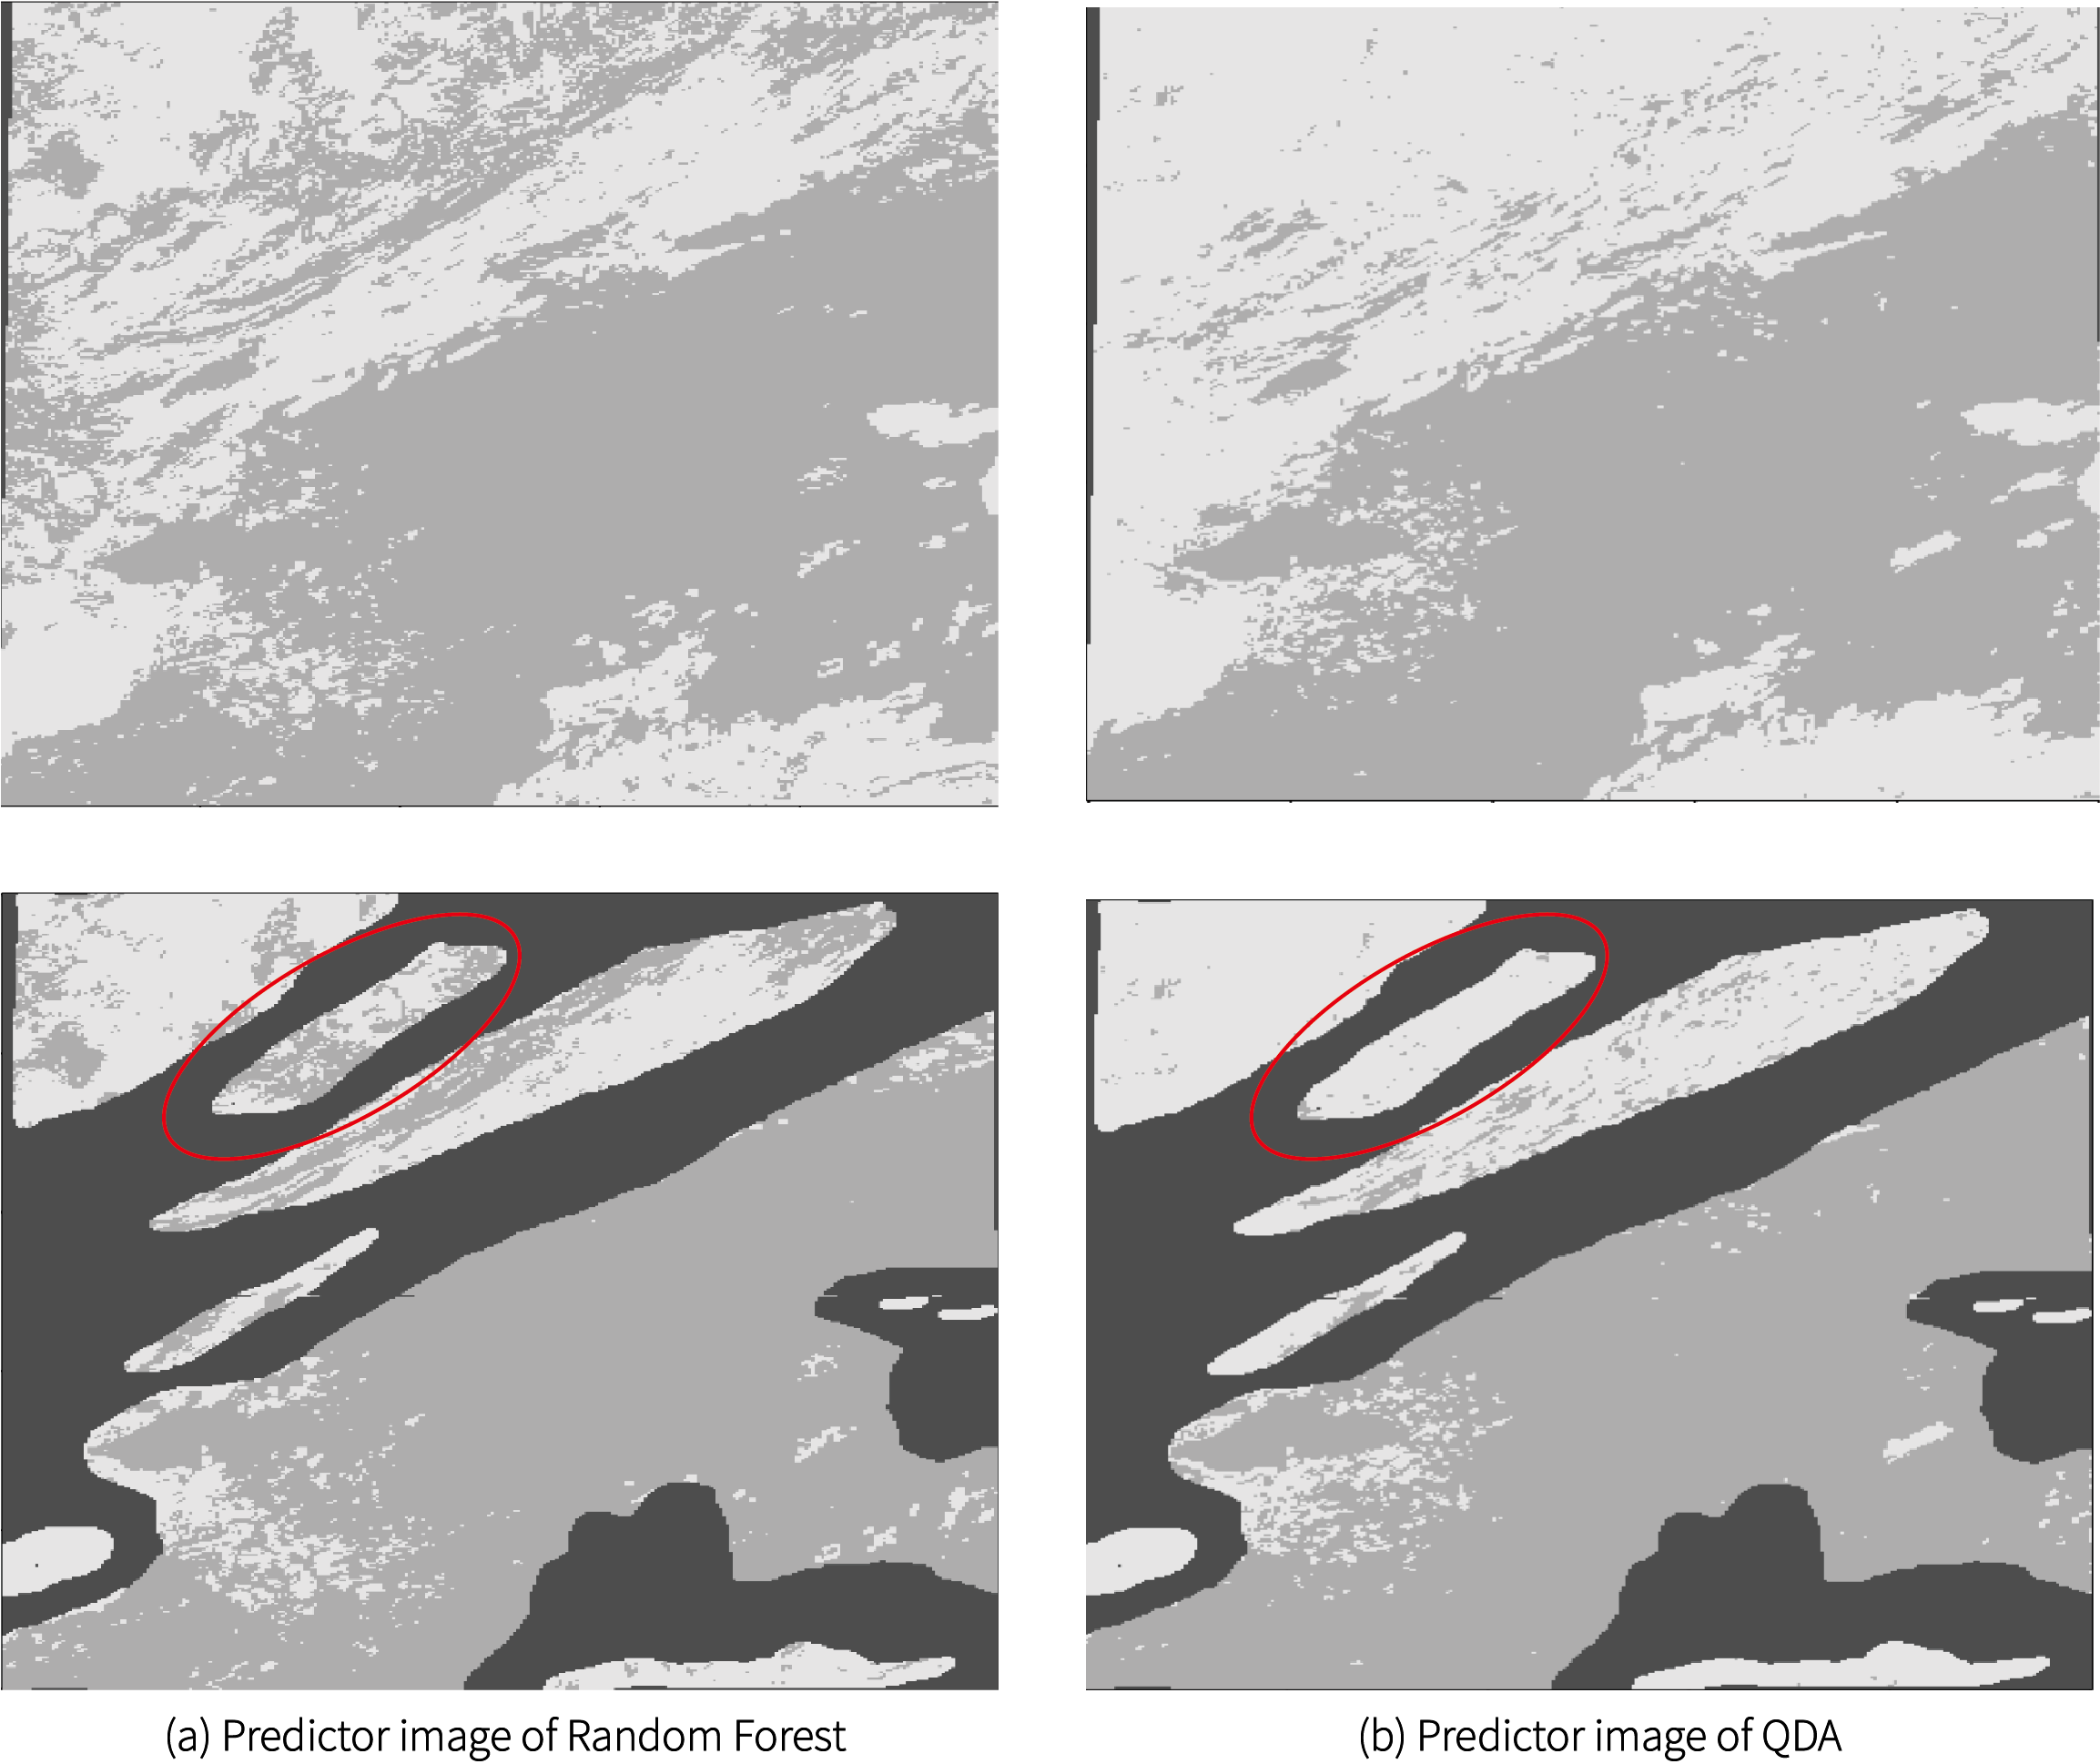
\includegraphics[width=0.6\columnwidth]{perform2.png} % Example image
	\caption{Performance of RF and QDA in data splitted by IBM}
\end{figure}

\subsection{Better classification (answer of -c-)}
In terms of the misclassification errors near the boundaries, we introduce a new indicator \textbf{score} to justify whether or not the pixel should be classified to the other group considering the correlation between neighbored pixels. The value of score $S_{ij}$ in pixel with $x=i,y=j$ is given by

$$
S_{ij} = \frac{\sum_{m=1-l}^{i+l}\limits\sum_{n=j-l}^{j+l}\hat{P}(y=1 | x)_{mn}}{l^2}\hat{y}_{ij}
$$

where $l$ refers to the window length.

If $S_{ij} < Threshold$, we take the classification of pixel $(i,j)$  $\hat{y}_{ij}$to be wrong and turn it into $-\hat{y}_{ij}$. The threshold is obtained through cross validation and control the intensification of aggregation of pixels in same group.

\begin{figure}[htb]
	\centering
	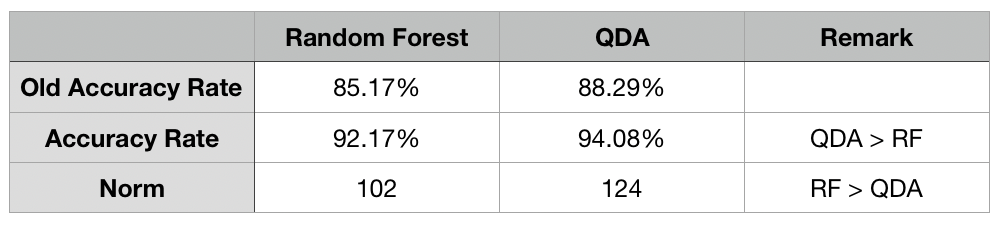
\includegraphics[width=0.8\columnwidth]{evaluate.png} % Example image
	\caption{Evaluation of RF and QDA after optimization}
\end{figure}

\begin{figure}[htb]
	\centering
	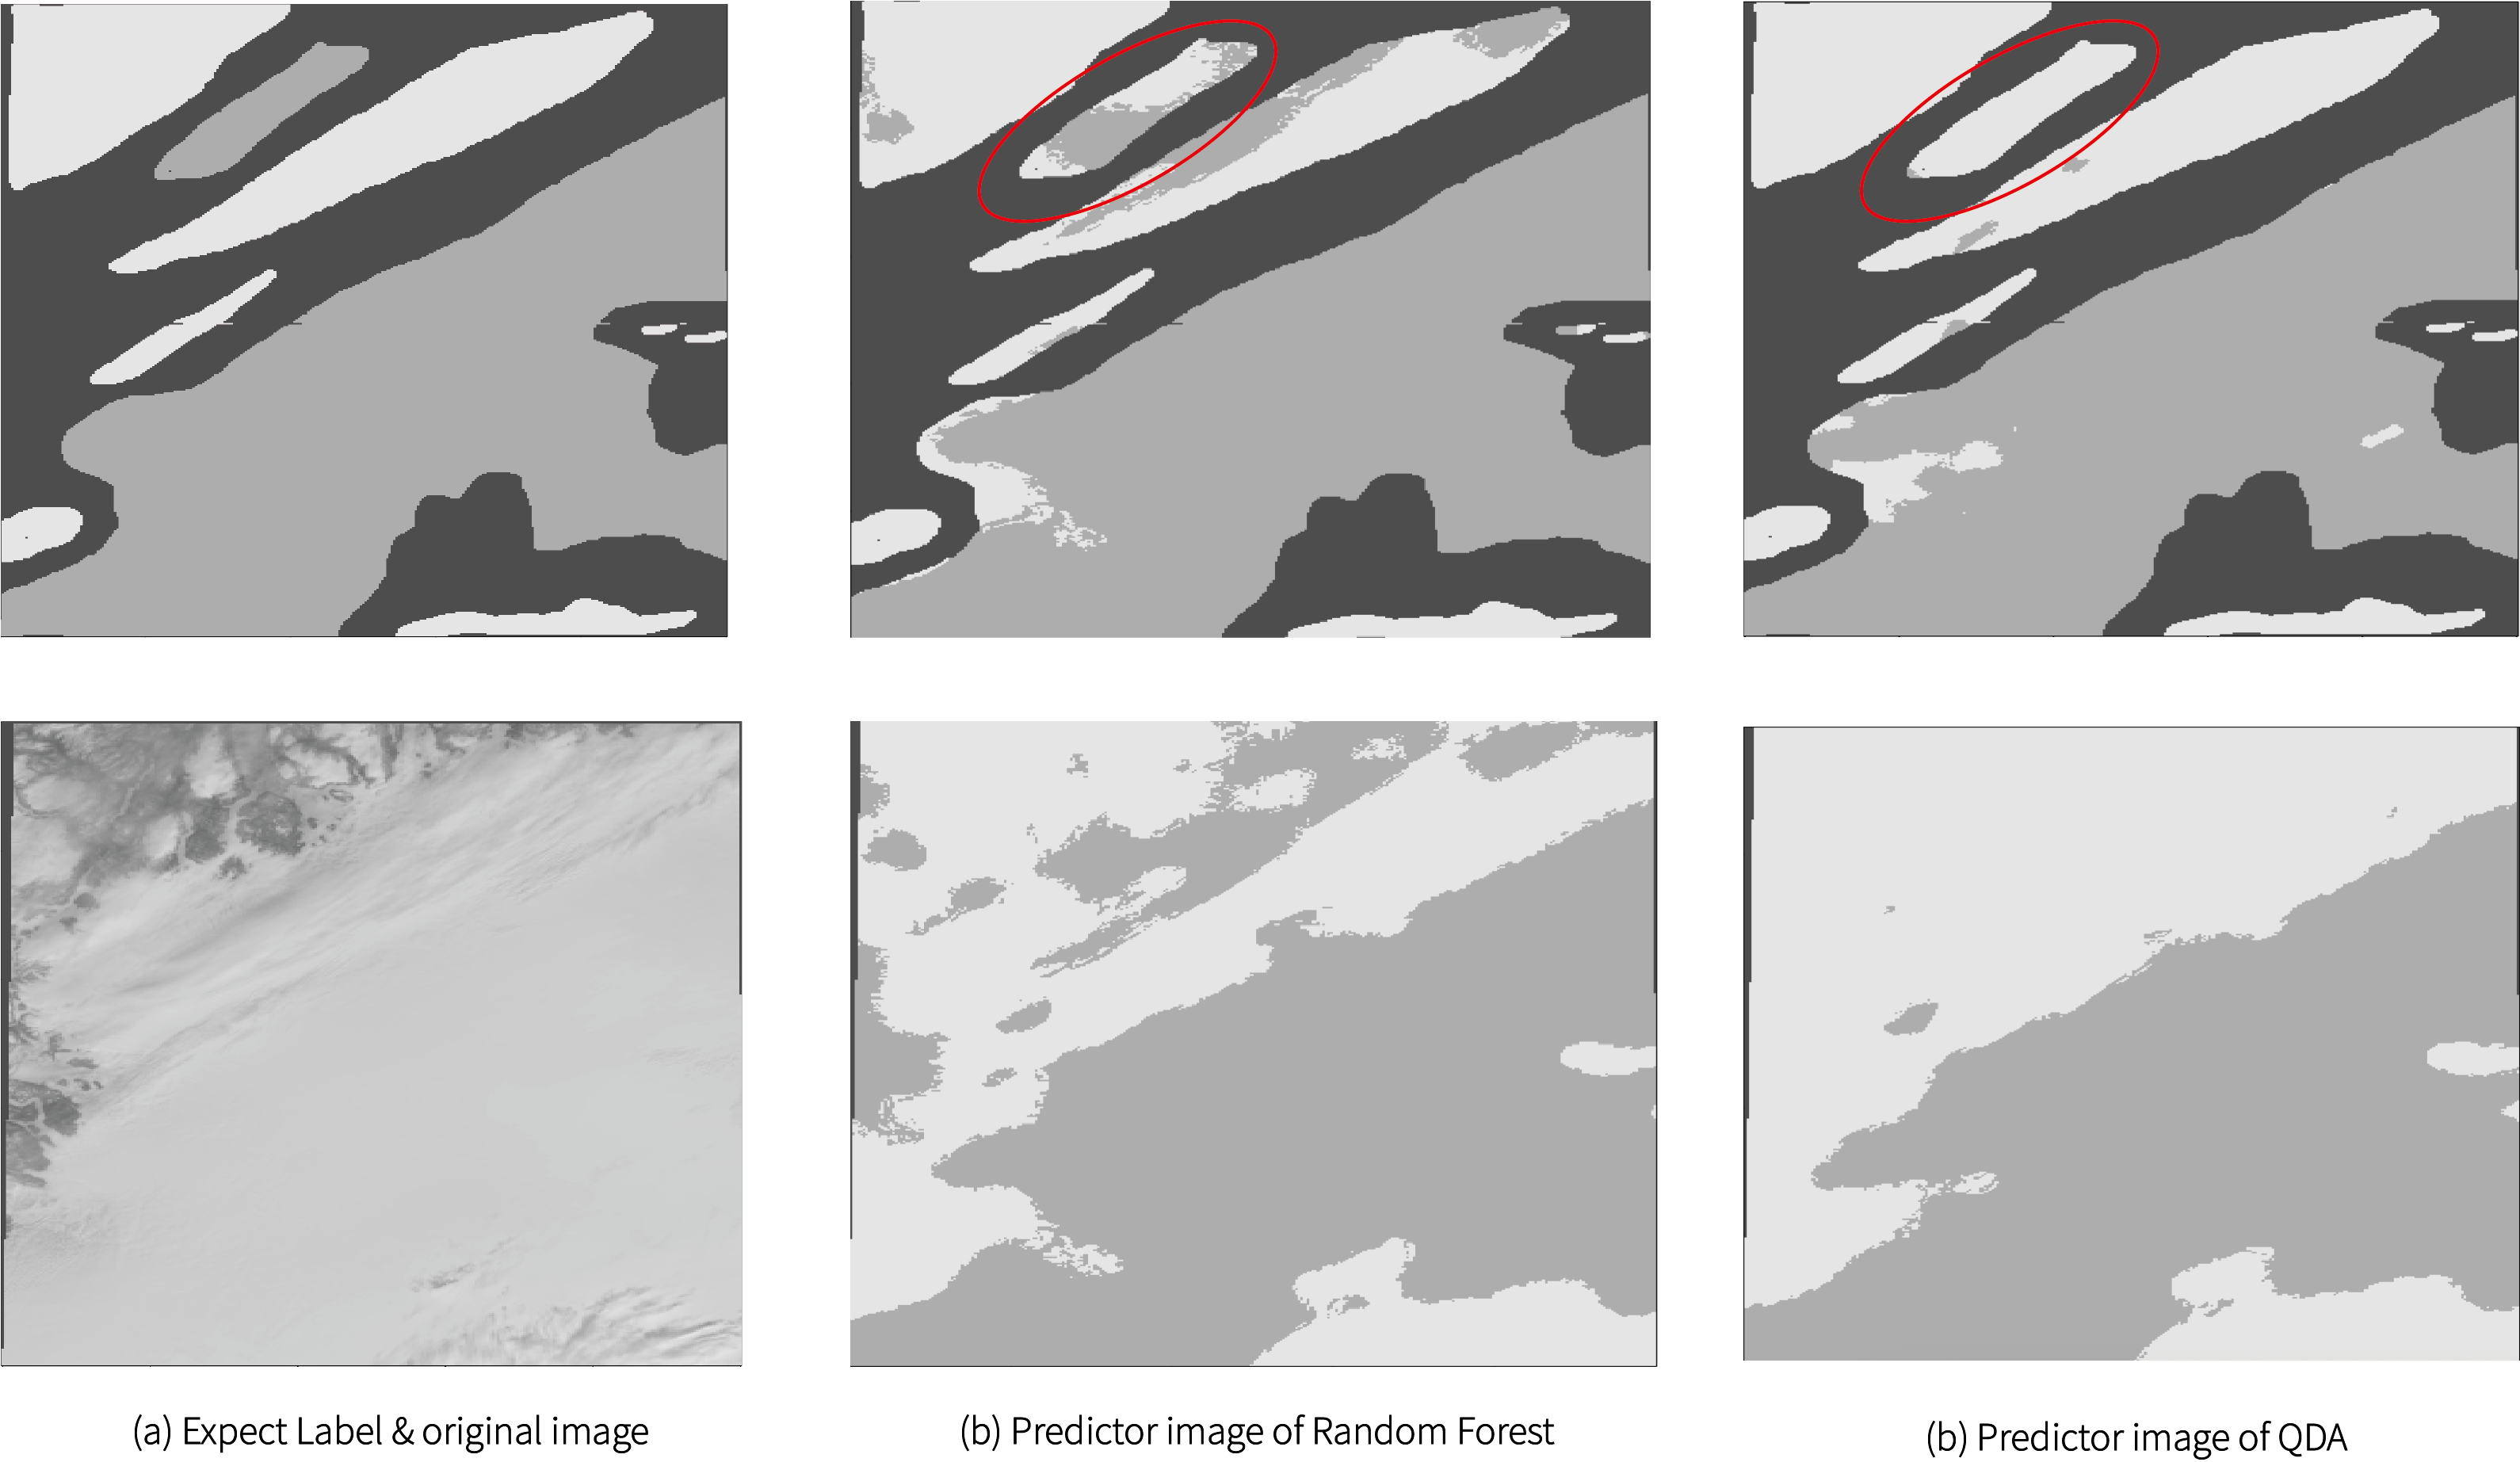
\includegraphics[width=0.8\columnwidth]{PoCMS.png} % Example image
	\caption{Performance of RF and QDA after optimization}
\end{figure}



As indicated in  figure 4.3, after optimized, the accurary of random forest is increased to 92.1\% , almost the same as the accuracy attained by QDA. But according to our new assessment method in section 3.3, the norm of random forest is 102 while that of QDA is 124, which indicates correctly that random forest perform better. The performance of this optimized classification method is showed in figure 4.4. As we can see, after optimization, the mis-classification errors near boundaries are greatly reduced while the regions marked by red circle which can not be correctly classified by QDA could be successfully identified mostly.  \\

In consideration for future data, our classification would fit well since we've already taken whole pictures as training set in our second splitting method and yield good results after normalizing features and optimizing the classification method in terms of the errors near boundaries.


\subsection{Conclusion}

\begin{enumerate}
   \item The second splitting method \textbf{Image Based Method} is of more practical meaning than the first method, though  with lower accuracy, since it is applied to data by picture as a whole instead of by picked pixel grid and thus more applicable for future data.
   \item Under the second splitting method, the Random forest classification perform very well in some specific regions where all other methods fail, and though its accuracy is not the highest (which is obtained by QDA method), the errors mainly occur near boundaries which can be smoothed and thus the accuracy would increase.
   \item The optimization method applied to random forest classification is to increase its accuracy based on the expert labels. But the smoothing may be not that pragmatic since the experts tend to give labels to entire regions while in fact there are always cloud and not cloud small areas in an entire region.
\end{enumerate}

\section{Contribution}

\begin{figure}[htb]
	\centering
	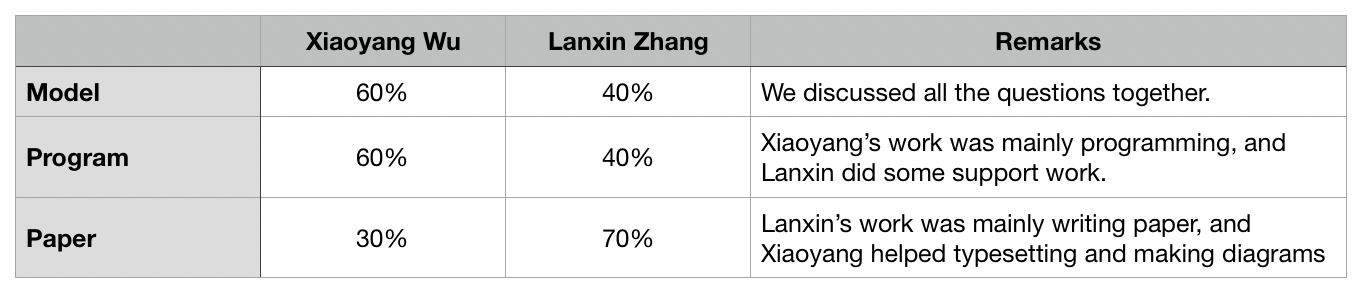
\includegraphics[width=1\columnwidth]{contri.png} % Example image
	\caption{Contribution Table}
\end{figure}

\end{document}
